\documentclass{article}

\usepackage{graphicx}
\usepackage{tikz}
\usepackage{tikzsymbols}
\usetikzlibrary{calc,patterns,shapes.geometric}
\pagestyle{empty}
\usepackage[margin=0pt]{geometry}
\geometry{papersize={14in,12in}}

\def\centerarc[#1](#2)(#3:#4:#5){\draw[#1] ($(#2)+({#5*cos(#3)},{#5*sin(#3)})$) arc (#3:#4:#5);}

\begin{document}
	\begin{figure}
		\centering
		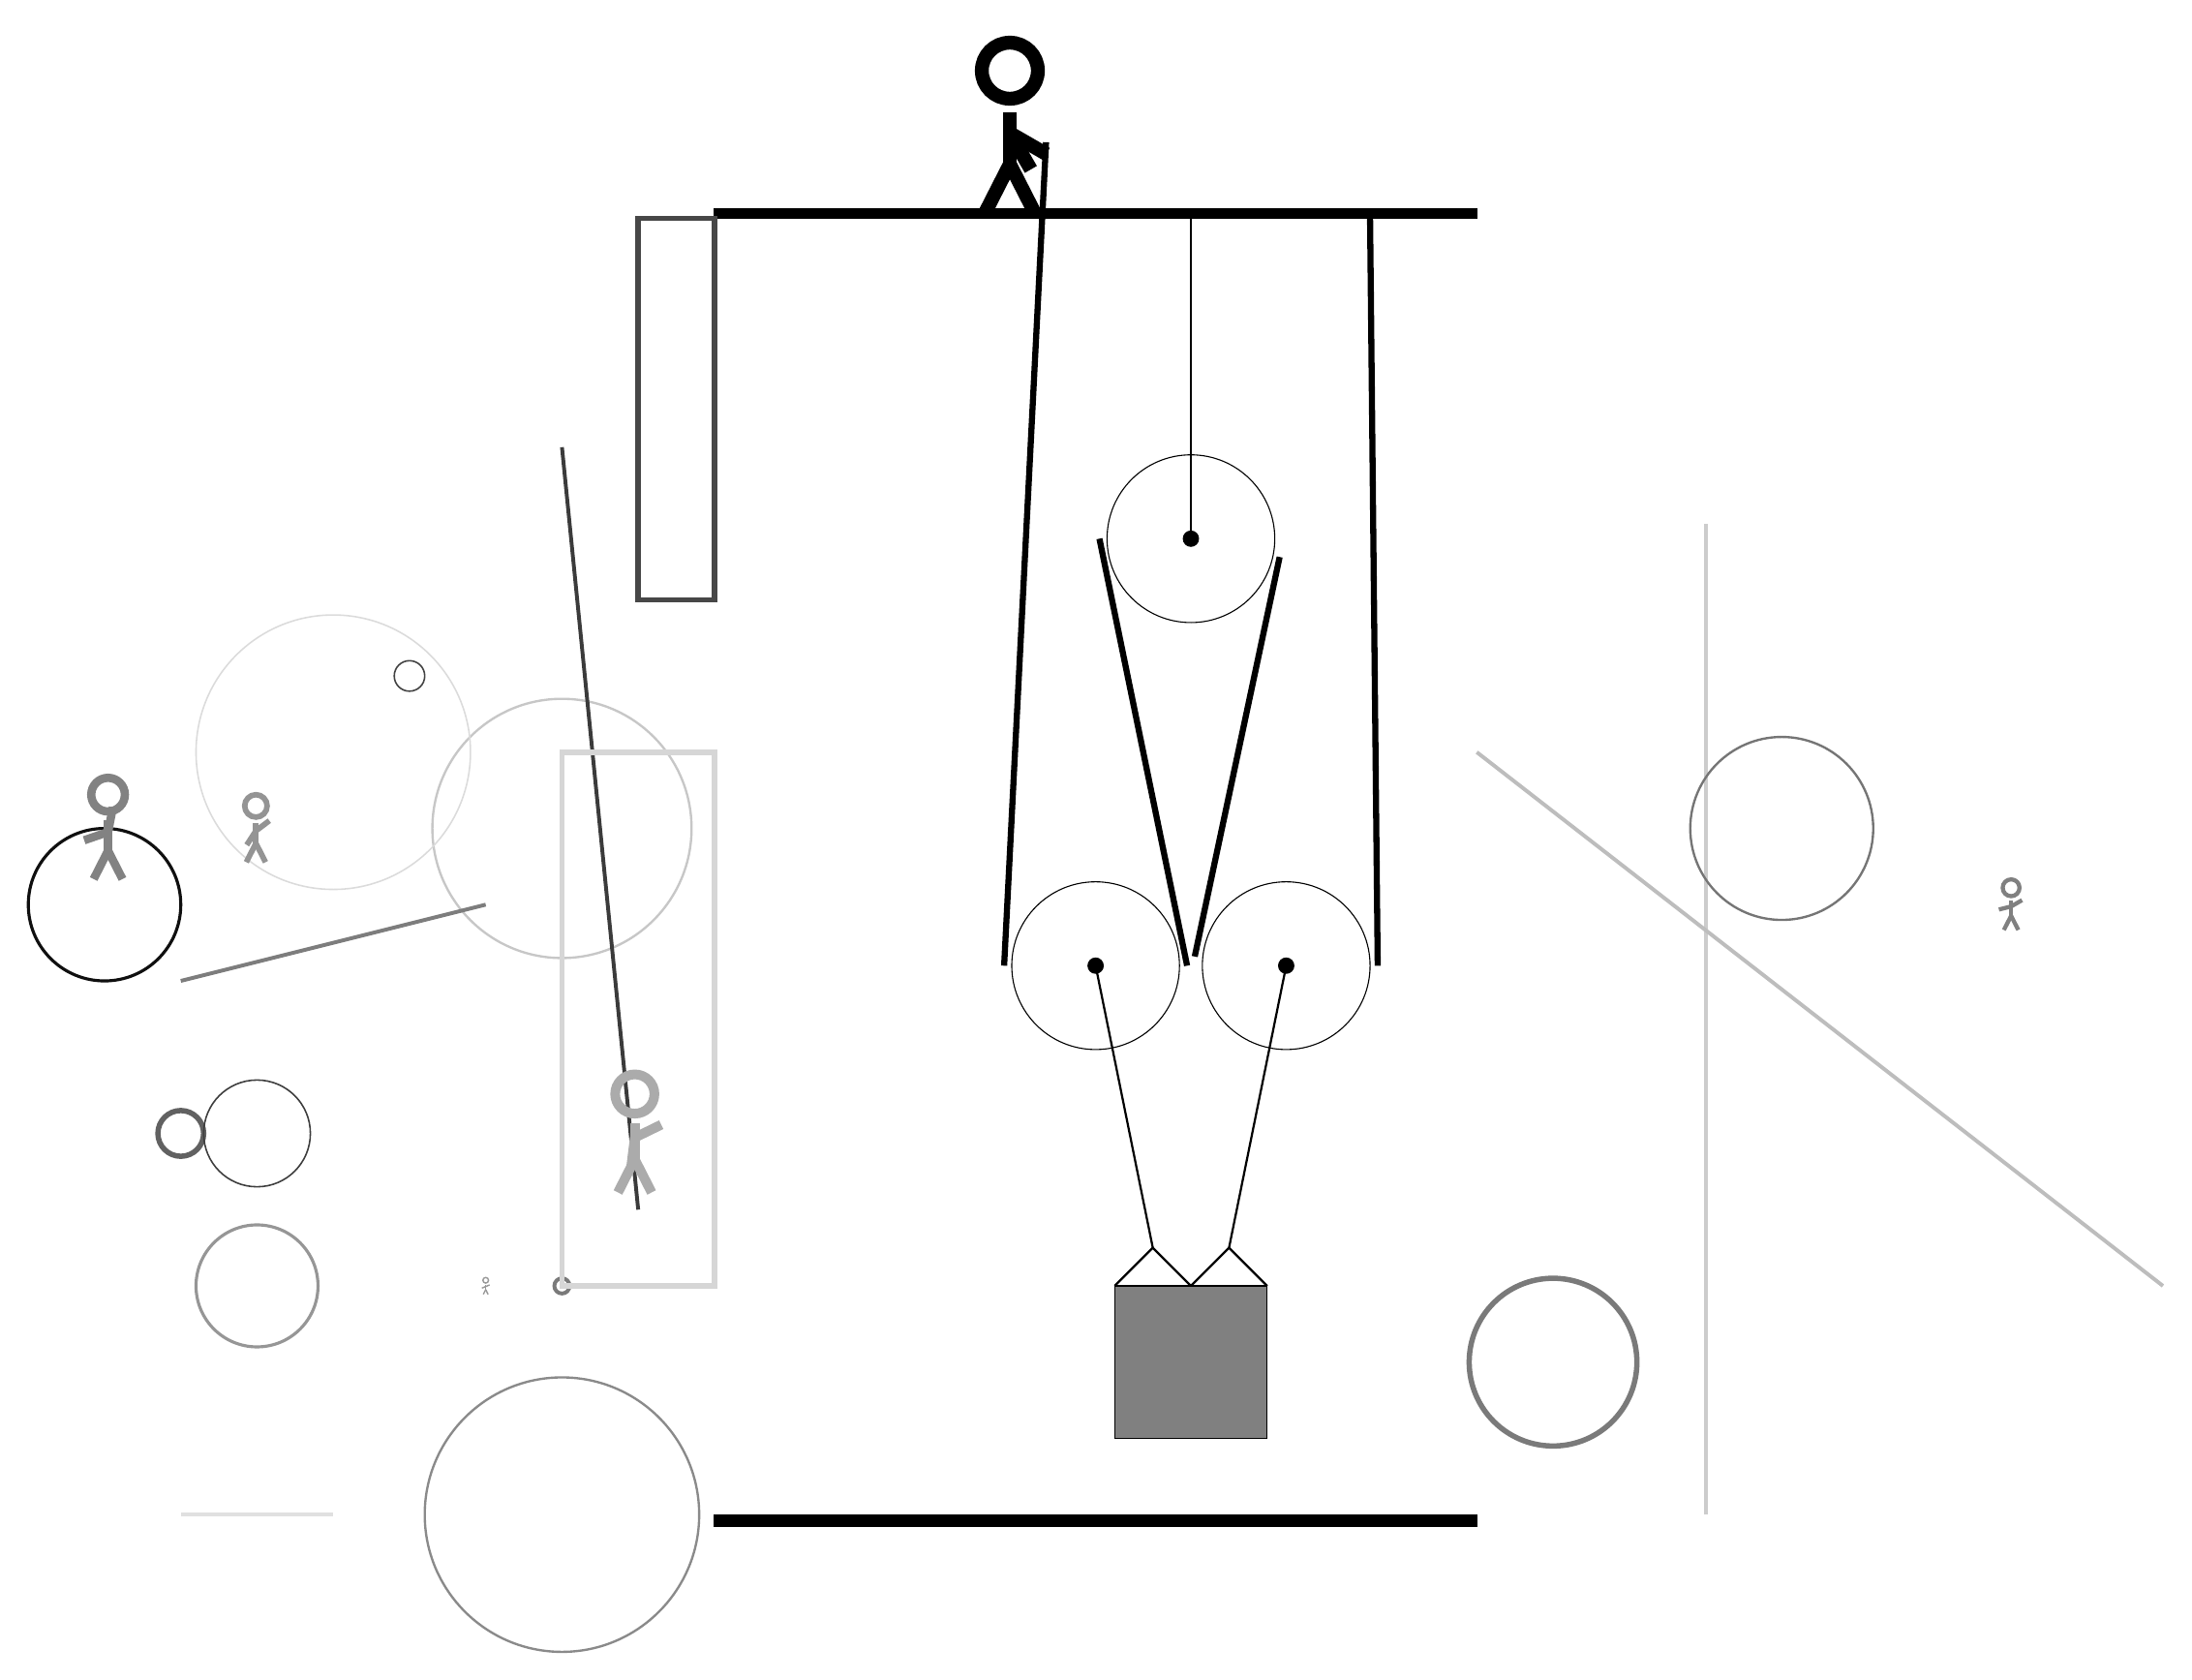
\begin{tikzpicture}
			%%%%% START %%%%%
			
			\draw[fill=black] (-4, 14) rectangle (6, 14.125);
			
			\draw (1, 4.2) circle (1.1);
			\draw[fill=black] (1, 4.2) circle (0.1);
			
			\draw (2.25, 9.8) circle (1.1);
			\draw[fill=black] (2.25, 9.8) circle (0.1);
			\draw[thick] (2.25, 9.8) -- (2.25, 14);
			
			\draw (3.5, 4.2) circle (1.1);
			\draw[fill=black] (3.5, 4.2) circle (0.1);
			
			\draw [line width=0.3mm, color=black!22](-6, 6) circle (1.7);
			
			\draw[line width=0.5mm, color=black!12](-9, -3) -- (-11, -3);
			\node[line width=0.2mm, color=black!50] at (13, 5) {\Strichmaxerl[3][14][30]};
			\draw[line width=0.5mm, color=black!77](-5, 1) -- (-6, 11);
			\draw [line width=0.4mm, color=black!94](-12, 5) circle (1.0);
			
			\draw [line width=0.2mm, color=black!14](-9, 7) circle (1.8);
			
			\draw [line width=0.5mm, color=black!52](-6, 0) circle (0.1);
			
			\draw [line width=0.7mm, color=black!62](-11, 2) circle (0.3);
			\draw[line width=0.7mm, color=black!72] (-4, 9) rectangle (-5, 14);
			\draw [line width=0.2mm, color=black!76](-10, 2) circle (0.7);
			\draw [line width=0.3mm, color=black!46](-6, -3) circle (1.8);
			
			\node[line width=0.7mm, color=black!40] at (-7, 0) {\Strichmaxerl[1][23][22]};
			\draw[line width=0.7mm, color=black!16] (-4, 7) rectangle (-6, 0);
			
			\draw[line width=0.5mm, color=black!20](9, -3) -- (9, 10);
			\node[line width=0.5mm, color=black!49] at (-12, 6) {\Strichmaxerl[6][19][79]};
			\draw [line width=0.2mm, color=black!74](-8, 8) circle (0.2);
			
			\draw[line width=0.5mm, color=black!51](-7, 5) -- (-11, 4);
			
			\draw [line width=0.7mm, color=black!52](7, -1) circle (1.1);
			\draw [line width=0.4mm, color=black!41](-10, 0) circle (0.8);
			\node[line width=0.4mm, color=black!33] at (-5, 2) {\Strichmaxerl[7][83][26]};
			\draw[line width=0.5mm, color=black!26](6, 7) -- (15, 0);
			\draw [line width=0.3mm, color=black!54](10, 6) circle (1.2);
			\node[line width=0.5mm, color=black!42] at (-10, 6) {\Strichmaxerl[4][57][37]};
			
			\draw[thick] (3.5, 4.2) -- (2.75, 0.5);
			\draw[thick] (1, 4.2) -- (1.75, 0.5);
			\draw[thick]  (1.25, 0) -- (1.75, 0.5) -- (2.25, 0);
			\draw[thick]  (2.25, 0) -- (2.75, 0.5) -- (3.25, 0);
			\draw[fill=black!50] (1.25, 0) rectangle (3.25, -2);
			
			\draw[line width=0.8mm] (0.35, 15) --  (-0.2, 4.2);
			\centerarc[line width=0.8mm](1, 4.2)(180:360:1.2000000000000002);
			\draw[line width=0.8mm] (2.2, 4.2) -- (1.05, 9.8);
			\centerarc[line width=0.8mm](2.25, 9.8)(-20:180:1.2000000000000002);
			\draw[line width=0.8mm](3.414, 9.56) -- (2.3, 4.32);
			\centerarc[line width=0.8mm](3.5, 4.2)(160:360:1.2000000000000002);
			\draw[line width=0.8mm](4.7, 4.2) -- (4.6, 14);
			
			\node at (-0.07, 15.2) {\Strichmaxerl[10][120][-30]};
			
			\draw[fill=black] (-4, -3) rectangle (6, -3.15);
			
			%%%%% END %%%%%
		\end{tikzpicture}
	\end{figure}	
\end{document}